\chapter{GIỚI THIỆU TỔNG QUAN}

\section{A/B Test}

A/B Testing (hay còn được gọi là split testing hay bucket testing) là một phương pháp để so sánh giữa 2 biến thể của một thuật toán hoặc ứng dụng nào đó, từ đó tìm ra được biến thể nào có hiệu quả tốt hơn.

\subsection{A/B Test là gì}

A/B Test chính là kỹ thuật chia đối tượng cần kiểm tra thành hai phiên bản A và B để đưa ra được phiên bản mà hiệu quả hơn thông qua kết quả tổng hợp với mỗi phiên bản đó.

A/B Test là cách viết tắt của một thử nghiệm ngẫu nhiên có đối chứng đơn giản, trong đó hai mẫu (A và B) của một biến vectơ duy nhất được so sánh. Các giá trị này tương tự nhau ngoại trừ một biến thể có thể ảnh hưởng đến hành vi của thuật toán. A/B Test được coi là hình thức đơn giản nhất của thử nghiệm có đối chứng. Tuy nhiên, bằng cách thêm nhiều biến thể hơn vào thử nghiệm, độ phức tạp của nó sẽ tăng lên.

A/B Test hữu ích để hiểu mức độ tương tác của người dùng và mức độ hài lòng của các tính năng trực tuyến như một tính năng hoặc sản phẩm mới. Các trang web truyền thông xã hội lớn như LinkedIn, Facebook và Instagram sử dụng A/B Test để làm cho trải nghiệm người dùng thành công hơn và như một cách để hợp lý hóa dịch vụ của họ.

Ngày nay, các A/B Test cũng đang được sử dụng để thực hiện các thử nghiệm phức tạp trên các chủ đề như hiệu ứng mạng khi người dùng ngoại tuyến, cách các dịch vụ trực tuyến ảnh hưởng đến hành động của người dùng và cách người dùng ảnh hưởng đến nhau. Nhiều ngành nghề sử dụng dữ liệu từ các bài kiểm tra A/B. Điều này bao gồm các kỹ sư dữ liệu, nhà tiếp thị, nhà thiết kế, kỹ sư phần mềm và doanh nhân. Nhiều vị trí dựa vào dữ liệu từ các A/B Test, vì chúng cho phép các công ty hiểu được sự tăng trưởng, tăng doanh thu và tối ưu hóa sự hài lòng của khách hàng.

Phiên bản A có thể là phiên bản được sử dụng hiện tại (do đó tạo thành nhóm gốc), trong khi phiên bản B được sửa đổi ở một số khía cạnh so với phiên bản A (do đó hình thành nhóm thử nghiệm). Ví dụ: trên một trang web thương mại điện tử, phễu mua hàng thường là một ứng cử viên tốt cho A/B Test, vì ngay cả tỷ lệ rớt hàng giảm nhẹ cũng có thể thể hiện mức tăng đáng kể trong bán hàng. Những cải tiến đáng kể đôi khi có thể được nhìn thấy thông qua các yếu tố thử nghiệm như bố cục, hình ảnh và màu sắc, nhưng không phải lúc nào cũng vậy. Trong các thử nghiệm này, người dùng chỉ thấy một trong hai phiên bản, vì mục đích là khám phá phiên bản nào trong hai phiên bản này thích hợp hơn.

\subsection{Cách A/B Test hoạt động}

Trong thử nghiệm A/B, bạn chụp một trang web hoặc màn hình ứng dụng và sửa đổi nó để tạo phiên bản thứ hai của cùng một trang. Thay đổi này có thể đơn giản như một dòng tiêu đề, một nút hoặc là một thiết kế lại hoàn toàn của trang. Sau đó, một nửa lưu lượng truy cập của bạn được hiển thị phiên bản gốc của trang (được gọi là điều khiển) và một nửa được hiển thị là phiên bản đã sửa đổi của trang (biến thể).

\begin{figure}[H]
	\centering
	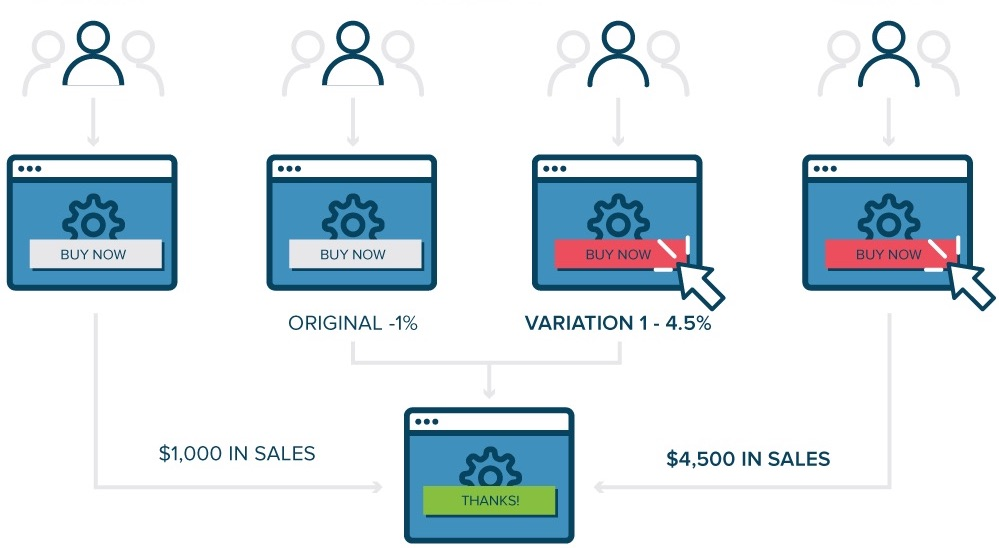
\includegraphics[height = 0.5\textwidth]{ab-testing-optimizely-2}
	\caption{A/B Test hoạt động như thế nào}
\end{figure}

Khi khách truy cập được phục vụ hoặc kiểm soát hoặc biến thể, mức độ tương tác của họ với từng trải nghiệm được đo lường và thu thập trong một bảng điều khiển và phân tích thông qua một công cụ thống kê. Sau đó, bạn có thể xác định xem việc thay đổi trải nghiệm có tác động tích cực, tiêu cực hay trung tính đến hành vi của khách truy cập hay không.

\begin{figure}[H]
	\centering
	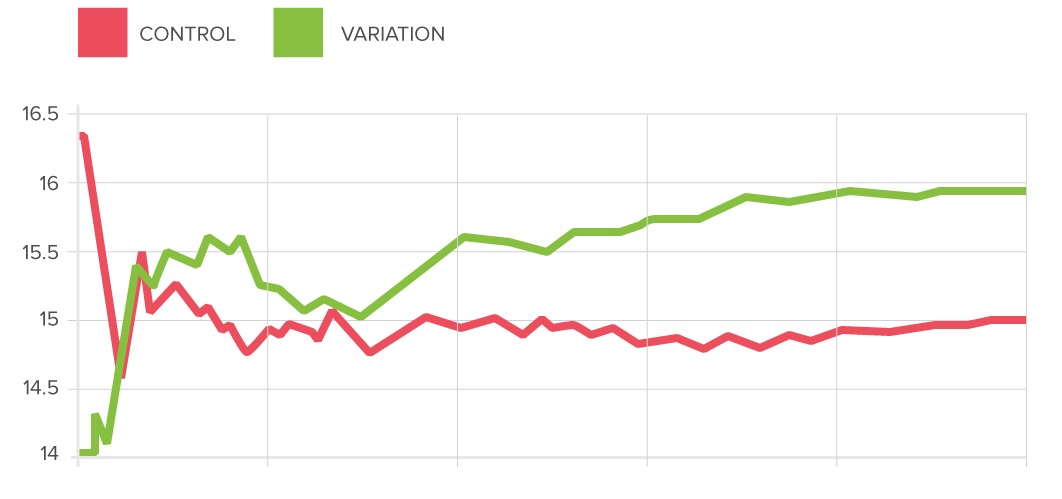
\includegraphics[height = 0.5\textwidth]{control-variation-graph-3}
	\caption{Biểu đồ so sánh kết quả các biến thể}
\end{figure}

\subsection{Ứng dụng của A/B Test}

A/B Test tăng trải nghiệm người dùng, giúp quảng cáo online thu thập được các dữ liệu lý tưởng. Họ sẽ hiểu hơn về hành vi quảng cáo nào ảnh hưởng đến người dùng để cung cấp các dịch vụ tốt nhất.

A/B Test giúp giảm tiền vào đầu tư các chiến dịch marketing. Chi phí thử nghiệm thấp nhưng hiệu quả mang về lại rất cao. Sales và marketing sẽ kết nối với nhau để tương tác hoạt động tốt hơn.

Xu hướng marketing online hiện nay đều chú trọng đến A/B Test. Chạy A/B Test cũng là một cách để kiểm tra cạnh tranh tốt hơn với các đối thủ. Để công việc kinh doanh của mình thành công bạn nên nghiên cứu về những lĩnh vực thử nghiệm này. Chúng sẽ giúp bạn thấu hiểu khách hàng, biết được hành vi của khách hàng để đưa ra các chiến lược kinh doanh quan trọng hơn.

\subsubsection{Đối với website}

Để tìm ra giao diện mà thu hút người sử dụng hơn thì chúng ta có thử nghiệm 2 phiên bản của giao diện đó, hai phiên bản sẽ khác nhau ở cách bố trí nội dung, vị trí đặt các button điều hướng, các hình ảnh, .....

\subsubsection{Đối với Email Marketing}

Đã qua rồi cái thời mà đẩy hàng trăm ngàn email đi và nghĩ rằng người dùng sẽ đọc được những email của mình gửi. Các email clients ngày càng có các bộ lọc tinh xảo hơn, tống tất cả các spam email vào thùng rác. Điều quan trọng là làm thế nào để khách hàng chịu mở email của mình ra xem và tương tác với các email đó. Câu trả lời chính là A/B Test.

Bạn có thể làm A/B Test để xác định được ngày nào trong tuần tỉ lệ mở mail cao nhất, gửi thời gian nào trong ngày là tốt nhất cho nội dung của bạn, tiêu đề email nào sẽ mang lại tỉ lệ mở mail cao hơn?...

\subsubsection{Đối với quảng cáo và bán hàng}

Đối với mảng online thì A/B Test thường được dùng để đo lường hiệu quả của các mẫu quảng cáo khác nhau. Ví dụ như khi bạn viết quảng cáo Adwords cho cùng 1 nhóm từ khóa (ad group) thì bạn nên viết 2 mẫu quảng cáo khác nhau và cho chạy song song để biết mẫu quảng cáo nào hiệu quả hơn sau một thời gian chạy. Tương tự với quảng cáo cho Facebook, sử dụng các thiết kế quảng cáo khác nhau cho cùng một chiến dịch để đo lường hiệu quả sau đó chọn mẫu thiết kế nào hiệu quả hơn để chạy tiếp. Việc tối ưu hóa quảng cáo thường xuyên bằng cách test các lựa chọn khác nhau sẽ giúp bạn liên tục cải thiện được tỷ lệ chuyển đổi và giúp quảng cáo chạy ngày càng hiệu quả hơn.

Đối với mảng offline thì A/B Test thường có thể được dùng để đánh giá hiệu quả của các kênh quảng cáo như báo giấy, tờ rơi, billboard… Chẳng hạn bằng cách sử dụng các mã coupon khác nhau cho từng mẫu quảng cáo trên báo, mẫu tờ rời, hoặc billboard, nhà quảng cáo có thể nắm được mẫu quảng cáo nào hiệu quả hơn thông qua việc có nhiều người sử dụng mã coupon nào hơn.

\subsubsection{Đối với ứng dụng di động}

A/B Test cũng được ứng dụng trong việc phát triển ứng dụng di động và tương tự như website, chủ yếu nhằm cải thiện UI/UX của sản phẩm.

Với các ứng dụng điện thoại di động thì việc tiến hành test thường khó khăn hơn nhiều cả về mặt kỹ thuật lẫn về hành vi người dùng.

Về mặt kỹ thuật thì để tiến hành test, thì phiên bản ứng dụng cần được cập nhật, được duyệt bởi AppStore hay Google Play rồi mới đến với người dùng do đó tốn nhiều thời gian hơn.

Về phương diện hành vi người dùng, không phải ai cũng sẽ cập nhật ngay phiên bản mới và trải nghiệm người dùng trên điện thoại di động hoàn toàn khác so với trên web.

\subsection{Quy trình thử nghiệm A/B}

Sau đây là khung thử nghiệm A/B mà có thể sử dụng để bắt đầu chạy thử nghiệm:

\begin{itemize}
	\bfitem {Thu thập dữ liệu}{Các phân tích của bạn thường sẽ cung cấp thông tin chi tiết về nơi bạn có thể bắt đầu tối ưu hóa. Nó hữu ích để bắt đầu với các khu vực có lưu lượng truy cập cao trên trang web hoặc ứng dụng của bạn để cho phép bạn thu thập dữ liệu nhanh hơn. Tìm kiếm các trang có tỷ lệ chuyển đổi thấp hoặc tỷ lệ rớt mạng cao có thể được cải thiện.}
	\bfitem {Xác định mục tiêu}{Mục tiêu chuyển đổi của bạn là số liệu mà bạn đang sử dụng để xác định xem biến thể có thành công hơn phiên bản gốc hay không. Mục tiêu có thể là bất cứ điều gì từ việc nhấp vào nút hoặc liên kết đến việc mua sản phẩm và đăng ký e-mail.}
	\bfitem {Tạo giả thuyết}{ Khi bạn đã xác định được mục tiêu, bạn có thể bắt đầu tạo ra các ý tưởng và giả thuyết thử nghiệm A/B để biết lý do tại sao bạn cho rằng chúng sẽ tốt hơn phiên bản hiện tại. Khi bạn đã có danh sách các ý tưởng, hãy sắp xếp thứ tự ưu tiên cho chúng về tác động dự kiến và mức độ khó thực hiện.}
	\bfitem {Tạo các biến thể}{Sử dụng phần mềm thử nghiệm A/B của bạn (như Optimizely), thực hiện các thay đổi mong muốn đối với một phần tử của trang web hoặc trải nghiệm ứng dụng dành cho thiết bị di động của bạn. Điều này có thể là thay đổi màu của nút, hoán đổi thứ tự của các phần tử trên trang, ẩn các phần tử điều hướng hoặc một cái gì đó hoàn toàn tùy chỉnh. Nhiều công cụ kiểm tra A/B hàng đầu có trình chỉnh sửa trực quan sẽ giúp những thay đổi này trở nên dễ dàng. Đảm bảo QA thử nghiệm của bạn để đảm bảo thử nghiệm hoạt động như mong đợi.}
	\bfitem {Chạy thử nghiệm}{Bắt đầu thử nghiệm của bạn và đợi khách tham gia! Tại thời điểm này, khách truy cập vào trang web hoặc ứng dụng của bạn sẽ được chỉ định ngẫu nhiên cho quyền kiểm soát hoặc biến thể trải nghiệm của bạn. Tương tác của họ với từng trải nghiệm được đo lường, tính toán và so sánh để xác định cách mỗi trải nghiệm hoạt động.}
	\bfitem {Phân tích kết quả}{Sau khi thử nghiệm của bạn hoàn tất, đã đến lúc phân tích kết quả. Phần mềm thử nghiệm A/B của bạn sẽ trình bày dữ liệu từ thử nghiệm và cho bạn thấy sự khác biệt giữa hai phiên bản trang của bạn hoạt động như thế nào và liệu có sự khác biệt có ý nghĩa thống kê hay không.}
\end{itemize}

\begin{figure}[H]
	\centering
	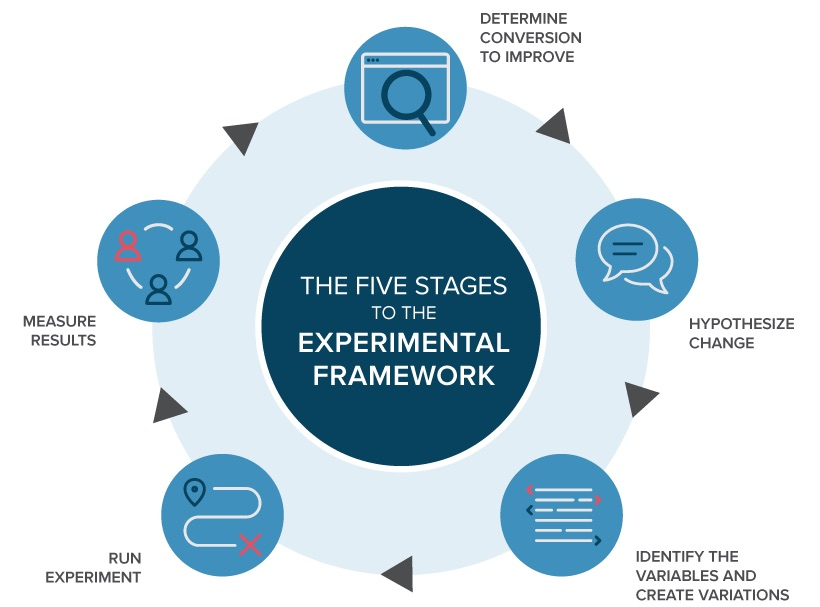
\includegraphics[height = 0.5\textwidth]{ab-testing-process-6}
	\caption{Quy trình thử nghiệm A/B}
\end{figure}

\section{Thông số của A/B Test trong Quảng Cáo}

\subsection{Tỷ lệ chuyển đổi (Conversion Rate)}

Hiểu một cách đơn giản, tỷ lệ chuyển đổi chính là tỷ lệ người truy cập vào website đã thực hiện hành động bạn mong muốn (click vào một trang quảng cáo, mua hàng, hay điền form khảo sát,....) trên tổng số lượt truy cập vào website

\begin{displaymath}
	CR = \frac{Conversions}{Clicks} * 100\%
\end{displaymath}

Lấy một ví dụ đơn giản như: Bạn có một website bán hàng, bạn muốn có thật nhiều người mua hàng trên website của bạn. Hôm nay website của bạn có 200 lượt truy cập trong đó có 5 lượt mua hàng thông qua website của bạn, khi đó bạn sẽ có con số về tỷ lệ chuyển đổi là $CR = (5/200) * 100\% = 2,5\%$. Việc của bạn là phải có các chiến lược để con số này càng cao càng tốt.

Tỷ lệ chuyển đổi tương tự như chỉ số doanh thu tăng lên vì trong thương mại điện tử, một chuyển đổi tương đương với một lần bán hàng. Tuy nhiên, việc đếm số lượng bán hàng khác với tính toán doanh thu: doanh thu cao hơn không cho thấy hoạt động tăng lên bởi vì nó dựa trên lợi nhuận chứ không chỉ dựa trên số lượng bán hàng. Biên lợi nhuận lớn có thể làm sai lệch kết quả; ví dụ, một lần bán thêm duy nhất với tỷ suất lợi nhuận lớn có thể cho thấy doanh thu tăng lên. Việc tính doanh số bán hàng đơn giản và rõ ràng hơn, nhưng điểm mạnh của nó cũng chứa một điểm yếu, như bạn sẽ thấy ở phần sau.

Lợi ích của việc sử dụng chuyển đổi làm phép đo là nó được tính ở quy mô nhỏ hơn: tìm kiếm. Do số lượng tìm kiếm dao động nhanh hơn số lượng chuyển đổi (khách hàng chuyển đổi ít thường xuyên hơn nhiều so với số lượng họ tìm kiếm), nên tỷ lệ tìm kiếm trên chuyển đổi có thể thay đổi nhanh chóng nếu khách hàng chuyển đổi thường xuyên hơn. Do đó, chuyển đổi có thể phát hiện các sửa đổi hệ thống dễ dàng hơn.

Do đó, tỷ lệ chuyển đổi ít mang tính định hướng hơn so với doanh thu nhưng có thể được phát hiện nhanh chóng - tức là tỷ lệ này nhạy cảm hơn. Thuộc tính này thích hợp hơn cho thử nghiệm A/B vì nó đạt được mức ý nghĩa nhanh hơn. Điều đó nói rằng, chuyển đổi không phải là một hình thức đo lường hoàn hảo vì nó coi tất cả doanh số bán hàng là bình đẳng, không mang lại giá trị kinh doanh giống nhau do tăng doanh thu.
\begin{figure}[H]
	\centering
	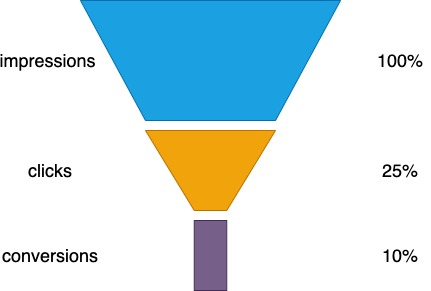
\includegraphics[height = 0.5\textwidth]{conversions}
	\caption{Conversions}
\end{figure}

\subsection{Tỷ lệ click (CTR)}

CTR là tỷ lệ cho biết tần suất những người xem quảng cáo hoặc danh sách sản phẩm sẽ nhấp vào quảng cáo hoặc danh sách sản phẩm miễn phí của bạn. Tỷ lệ nhấp (CTR) có thể được sử dụng để đánh giá mức độ hoạt động của các từ khóa và quảng cáo cũng như danh sách miễn phí của bạn.

CTR là số nhấp chuột mà quảng cáo của bạn nhận được chia cho số lần quảng cáo của bạn được hiển thị: nhấp chuột ÷ hiển thị = CTR. Ví dụ: nếu bạn có 5 nhấp chuột và 100 hiển thị, thì CTR của bạn sẽ là 5%.

\begin{displaymath}
	CTR = \frac{Clicks}{Impressions} * 100\%
\end{displaymath}

Mỗi quảng cáo, danh sách và từ khóa của bạn có CTR riêng mà bạn có thể thấy được liệt kê trong tài khoản của mình.

CTR cao là một dấu hiệu tốt cho thấy người dùng thấy quảng cáo và danh sách của bạn hữu ích và có liên quan. CTR cũng đóng góp vào CTR dự kiến của từ khóa của bạn, là một thành phần của Xếp hạng quảng cáo. Lưu ý rằng CTR tốt có liên quan đến những gì bạn đang quảng cáo và trên mạng nào.

Bạn có thể sử dụng CTR để đánh giá những quảng cáo, danh sách và từ khóa nào thành công với bạn và những quảng cáo nào cần được cải thiện. Từ khóa, quảng cáo và danh sách của bạn càng liên quan đến nhau và với doanh nghiệp của bạn, thì càng có nhiều khả năng người dùng nhấp vào quảng cáo hoặc danh sách của bạn sau khi tìm kiếm trên cụm từ khóa của bạn.

\section{Cấu trúc của A/B Test}

Một A/B Test được chia làm thành nhiều tầng lớp.  Mỗi tầng lớp đều có ý nghĩa riêng và được chia ra để có thể phục vụ cho logic business phức tạp.

\begin{figure}[H]
	\centering
	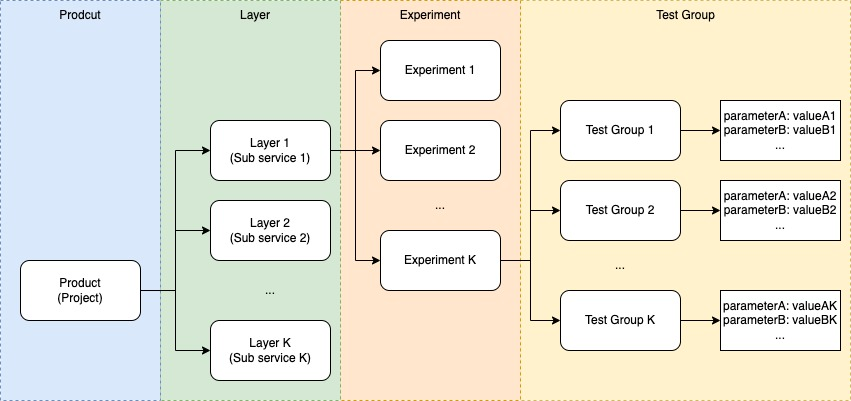
\includegraphics[height = 0.5\textwidth]{overview-ab-testing}
	\caption{Tổng quan của một A/B Test}
\end{figure}

\subsection{Product}

Product là thực thể cao nhất trong một A/B Test. Mỗi product thường đại diện cho một tập thể lớn. Mỗi team thường có nhiều bộ phận cho các lĩnh vực khác nhau, mỗi bộ phận sẽ thường có một hoặc nhiều Product.

Mỗi Product được chia ra để tách biệt các A/B Test giữa các team khác nhau. A/B Test thuộc hai Product khác nhau sẽ không liên quan gì đến nhau, không để so sánh được cùng với nhau.

\begin{figure}[H]
	\centering
	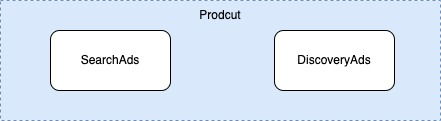
\includegraphics[width = 1\textwidth]{product}
	\caption{Product}
\end{figure}

Ví dụ: trong phòng quảng cáo thì sẽ có hai bộ phận lớn là quảng cáo tìm kiếm và quảng cáo gợi ý. Mỗi bộ phận sẽ có 2 product khác nhau để khi thực hiện A/B Test không ảnh hưởng lẫn nhau.

\subsection{Layer}

Layer là thực thể thức hai đứng sau thực thể Product. Mỗi Layer đại diện cho một logic nhỏ hơn của Product đấy. Một Product có thể có nhiều Layer.

Mỗi layer sẽ có tổng cộng 100\% lượng truy cập. Tầng sau sẽ sử dụng một lượng nhỏ truy cập trong 100\% lượng truy cập đấy.

Ngoài ra, với mỗi layer, có thể cài đặt layer này sử dụng một cơ số để phân chia lượng truy cập. Các cơ số có thể là:

\begin{itemize}
	\bfitem {request\_id}{sử dụng request\_id để phân chia truy cập.}
	\bfitem {user\_id}{sử dụng user\_id để phân chia truy cập.}
\end{itemize}

Khi một truy cập được gọi tới, truy cập đó sẽ đi qua từng Layer. Với mỗi layer, nó sẽ sử dụng cơ số để quyết định xem layer này sẽ sử dụng thí nghiệm nào.

\begin{figure}[H]
	\centering
	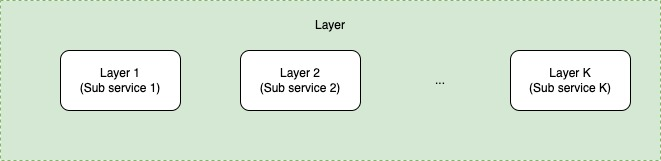
\includegraphics[width = 1\textwidth]{layer}
	\caption{Layer}
\end{figure}

\subsection{Experiment}

Experiment là thực thể tiếp theo đứng dưới một layer, mỗi experiment chỉ thuộc một layer. Một experiment chính là một thí nghiệm mà được tạo ra để thử nghiệm một mô hình tính toán mới. Ví dụ: thử nghiệm thuật toán A mới để tính toán giá cả, thử nghiệm giao dịch màu mới để tăng trải nghiệm người dùng, v.v.

Mỗi experiment sẽ quản lý trạng thái, thời gian bắt đầu và thời gian kết thúc của experiment đó. Ngoài ra, mỗi experiment sẽ chiếm một tỉ lệ phần trăm truy cập của một layer. Một layer có thể có nhiều experiment. Ví dụ: layer tính toán giá cả sẽ có hai thí nghiệm thử nghiệm hai thuật toán A và B, mỗi thuật toán có 10\% lượng truy cập để đánh giá.

Như vậy, với mỗi layer, khi một truy cập đi đến, nó sẽ sử dụng không hoặc một experiment bất kỳ dựa trên cơ số của layer đó. Mỗi truy cập đều có user\_id và request\_id đi kèm, layer sẽ sử dụng hai cơ số đó để quyết định Experiment nào sẽ được thực hiện.

\begin{figure}[H]
	\centering
	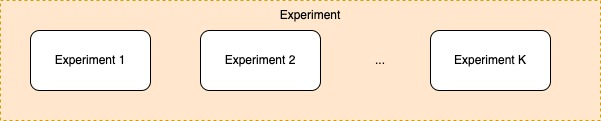
\includegraphics[width = 1\textwidth]{experiment}
	\caption{Experiment}
\end{figure}

\subsection{Test Group}

Test Group là thực thể nhỏ nhất trong một A/B Test. Test Group đại diện cho một biến thể của một Experiment. Ví dụ khi sử dụng thuật toán A để tính toán giá cả của sản phẩm, thuật toán A có thể sử dụng hai chỉ số khác nhau để tính toán tương ứng với hai test group khác nhau.

Khi thực hiện một Experiment, mỗi Test Group sẽ có một lượng truy cập giống nhau và kết quả sẽ được so sánh giữa hai Test Group. Ví dụ trong thuật toán A, hai biến thể X và Y sẽ có một biến thể mang lại kết quả tốt hơn khi so sánh với nhau.

\begin{figure}[H]
	\centering
	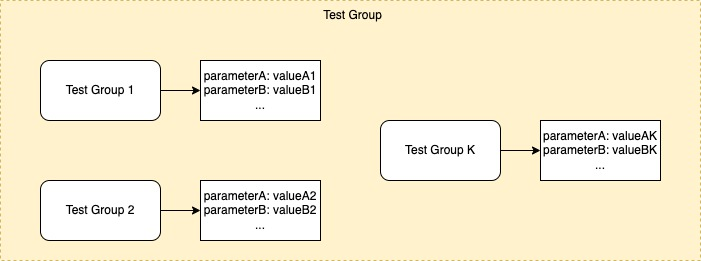
\includegraphics[width = 1\textwidth]{test-group}
	\caption{Test Group}
\end{figure}

\section{Công nghệ thực hiện}

\subsection{Golang}

\begin{figure}[H]
	\centering
	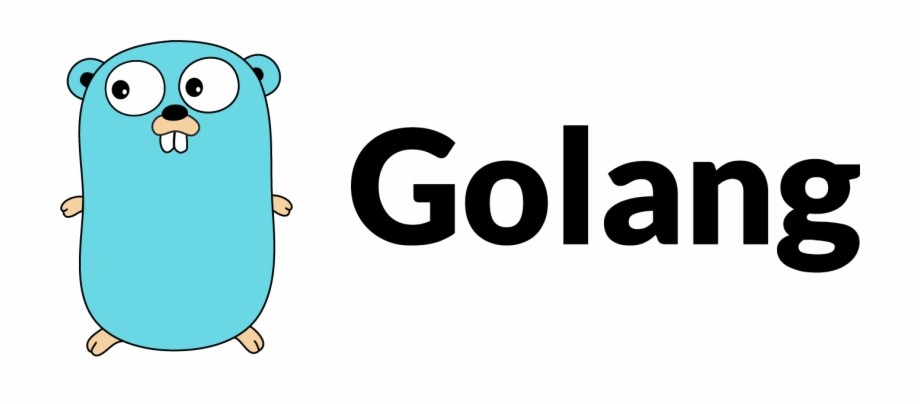
\includegraphics[height = 0.3\textwidth]{golang}
	\caption{Golang}
\end{figure}

Golang còn được gọi là Go là một ngôn ngữ lập trình open-source, compiled và statically-typed do Google phát triển.

Go là một ngôn ngữ lập trình đa năng với cú pháp đơn giản và một thư viện tiêu chuẩn mạnh mẽ. Go cải thiện các khái niệm như lập trình mệnh lệnh và hướng đối tượng và do đó đơn giản hóa môi trường làm việc cho các lập trình viên.

\subsubsection{Ưu điểm của Golang}

\begin{itemize}
	\bfitem {Cú pháp đơn giản}{Go có cú pháp ngắn gọn và đơn giản giúp viết mã dễ đọc và dễ bảo trì.}
	\bfitem {Liên kết tĩnh}{Trình biên dịch hỗ trợ liên kết tĩnh có nghĩa là bạn có thể liên kết tĩnh dự án của mình thành một tệp nhị phân lớn và sau đó chỉ cần triển khai nó lên máy chủ.}
	\bfitem {Ngôn ngữ Strong và Statically Type}{Strong có nghĩa là sau khi bạn tạo một số biến bằng cách sử dụng một số kiểu dữ liệu thì đối với toàn bộ ứng dụng, nó sẽ vẫn là kiểu dữ liệu đấy. Statically Type là tất cả các biến phải xác định tại thời điểm biên dịch.}
	\bfitem {Concurrency tích hợp}{Go có tính năng concurrency được tích hợp sẵn. Sử dụng Go Routines và các kênh, bạn có thể xử lý đồng thời các tác vụ rất dễ dàng và hiệu quả.}
\end{itemize}

\begin{figure}[H]
	\centering
	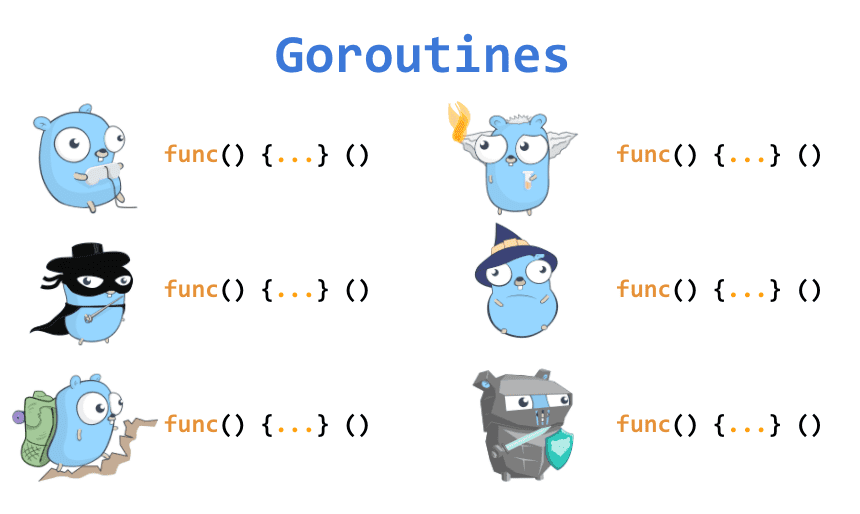
\includegraphics[height = 0.3\textwidth]{goroutines}
	\caption{Goroutine}
\end{figure}
\begin{figure}[H]
	\centering
	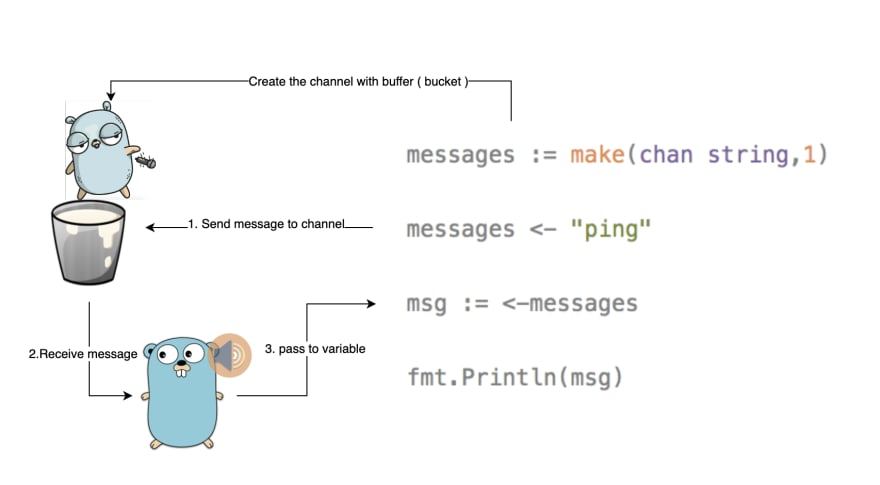
\includegraphics[height = 0.3\textwidth]{channel}
	\caption{Channel}
\end{figure}

\subsubsection{Ứng dụng của Golang}

\begin{itemize}
	\bfitem{Dịch vụ đám mây}{Go giúp các doanh nghiệp xây dựng và mở rộng quy mô hệ thống điện toán đám mây. Khi các ứng dụng và quá trình xử lý chuyển sang đám mây, đồng thời trở thành một vấn đề rất lớn. Về bản chất, các hệ thống điện toán đám mây chia sẻ và mở rộng quy mô tài nguyên. Điều phối quyền truy cập vào các tài nguyên được chia sẻ là một vấn đề ảnh hưởng đến mọi quá trình xử lý ứng dụng trên đám mây và yêu cầu ngôn ngữ lập trình “hướng đến phát triển các ứng dụng đồng thời có độ tin cậy cao”.}
	\bfitem {Command-line Interfaces (CLIs)}{Giao diện dòng lệnh (CLI), không giống như giao diện người dùng đồ họa (GUI), chỉ ở dạng văn bản. Các ứng dụng cơ sở hạ tầng và đám mây chủ yếu dựa trên CLI do khả năng tự động hóa và điều khiển từ xa dễ dàng.}
	\bfitem {Web Development}{Go được thiết kế để cho phép các nhà phát triển nhanh chóng phát triển các ứng dụng web có khả năng mở rộng và bảo mật. Go đi kèm với một máy chủ web dễ sử dụng, an toàn và hiệu quả và bao gồm thư viện tạo khuôn mẫu web riêng. Go có hỗ trợ tuyệt vời cho tất cả các công nghệ mới nhất từ HTTP / 2, cơ sở dữ liệu như MySQL, MongoDB và ElasticSearch, cho đến các tiêu chuẩn mã hóa mới nhất bao gồm TLS 1.3. Các ứng dụng web của Go chạy nguyên bản trên Google App Engine và Google Cloud Run (để dễ dàng mở rộng quy mô) hoặc trên bất kỳ môi trường, đám mây hoặc hệ điều hành nào nhờ tính di động cực cao của Go.}
	\bfitem {Development Operations \& Site Reliability Engineering}{Thời gian khởi động và xây dựng nhanh. Thư viện tiêu chuẩn mở rộng của Go — bao gồm các gói cho các nhu cầu thông thường như HTTP, I / O tệp, thời gian, biểu thức chính quy, thực thi và các định dạng JSON / CSV — cho phép DevOps / SRE đi đúng vào logic kinh doanh của họ. Ngoài ra, hệ thống kiểu tĩnh và xử lý lỗi rõ ràng của Go giúp các tập lệnh nhỏ thậm chí còn mạnh mẽ hơn.}
\end{itemize}

\subsection{React}

\begin{figure}[H]
	\centering
	
\includegraphics[height = 0.3\textwidth]{react}
	\caption{React}
\end{figure}

\subsubsection{React là gì}

React (còn được gọi là React.js hoặc ReactJS) là một thư viện JavaScript front-end mã nguồn mở và miễn phí để xây dựng giao diện người dùng dựa trên các thành phần UI. Nó được duy trì bởi Meta (trước đây là Facebook) và một cộng đồng các nhà phát triển và công ty cá nhân. React có thể được sử dụng làm cơ sở để phát triển các single-page, ứng dụng di động hoặc ứng dụng web với các framework như Next.js.

Tuy nhiên, React chỉ quan tâm đến việc quản lý trạng thái và hiển thị trạng thái đó cho DOM, vì vậy việc tạo các ứng dụng React thường yêu cầu sử dụng các thư viện bổ sung để định tuyến, cũng như một số chức năng phía client.

\subsubsection{Đặc trưng của React}

\textbf{Declarative}

React giúp tạo giao diện người dùng tương tác dễ dàng hơn. Thiết kế các khung nhìn đơn giản cho từng trạng thái trong ứng dụng của bạn và React sẽ cập nhật và hiển thị các thành phần phù hợp một cách hiệu quả khi dữ liệu của bạn thay đổi.

Chế độ xem Declarative làm cho code của bạn dễ đoán hơn và dễ debug hơn.

\textbf{Component-Based}

Xây dựng các thành phần được đóng gói quản lý trạng thái của riêng chúng, sau đó biên soạn chúng để tạo giao diện người dùng phức tạp.

Vì logic thành phần được viết bằng JavaScript thay vì các mẫu, bạn có thể dễ dàng chuyển dữ liệu phong phú thông qua ứng dụng của mình và giữ trạng thái không nằm trong DOM.

\textbf{Learn Once, Write Anywhere}

Chúng tôi không đưa ra giả định về phần còn lại của nền tảng công nghệ của bạn, vì vậy bạn có thể phát triển các tính năng mới trong React mà không cần viết lại mã hiện có.

React cũng có thể render trên server bằng Node và compile ra các ứng dụng di động bằng React Native.

\textbf{Virtual DOM}

\begin{figure}[H]
	\centering
	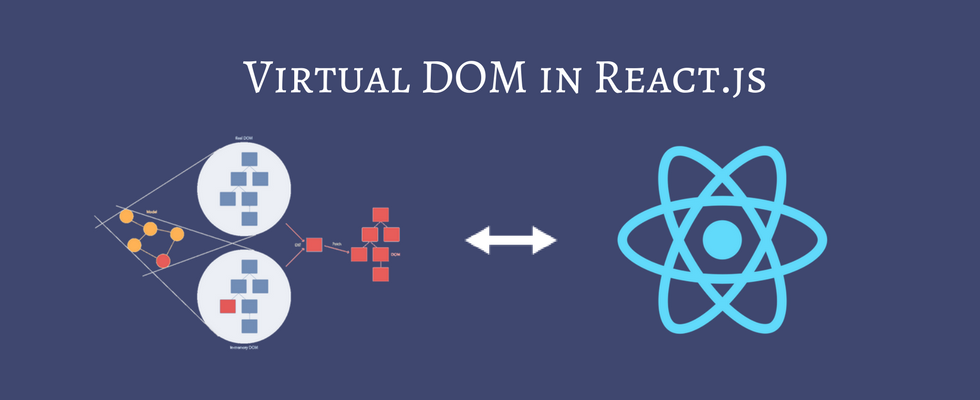
\includegraphics[height = 0.3\textwidth]{virtual-dom}
	\caption{Virtual DOM}
\end{figure}

Những Framework sử dụng Virtual-DOM như ReactJS khi Virtual-DOM thay đổi, chúng ta không cần thao tác trực tiếp với DOM trên View mà vẫn phản ánh được sự thay đổi đó. Do Virtual-DOM vừa đóng vai trò là Model, vừa đóng vai trò là View nên mọi sự thay đổi trên Model đã kéo theo sự thay đổi trên View và ngược lại. Có nghĩa là mặc dù chúng ta không tác động trực tiếp vào các phần tử DOM ở View nhưng vẫn thực hiện được cơ chế Data-binding. Điều này làm cho tốc độ ứng dụng tăng lên đáng kể – môt lợi thế không thể tuyệt vời hơn khi sử dụng Virtula-DOM.

\subsection{Redis}

\begin{figure}[H]
	\centering
	
\includegraphics[height = 0.3\textwidth]{redis}
	\caption{Redis}
\end{figure}

\subsubsection{Redis là gì}

Redis, viết tắt của Remote Dictionary Server, là một kho lưu trữ dữ liệu key-value, mã nguồn mở, in-memeory và nhanh chóng. Dự án bắt đầu khi Salvatore Sanfilippo, nhà phát triển ban đầu của Redis, muốn cải thiện khả năng mở rộng của công ty khởi nghiệp của mình. Từ đó, anh phát triển Redis, hiện được sử dụng làm cơ sở dữ liệu, bộ nhớ đệm, message broker và hàng đợi.

Redis cung cấp thời gian phản hồi dưới mili giây, cho phép hàng triệu yêu cầu mỗi giây cho các ứng dụng thời gian thực trong các ngành như trò chơi, công nghệ quảng cáo, dịch vụ tài chính, chăm sóc sức khỏe và IoT. Ngày nay, Redis là một trong những engine mã nguồn mở phổ biến nhất hiện nay, được Stack Overflow đặt tên là cơ sở dữ liệu "Được yêu thích nhất" trong 5 năm liên tiếp. Do hiệu suất nhanh, Redis là một lựa chọn phổ biến cho bộ nhớ đệm, quản lý phiên, chơi trò chơi, bảng xếp hạng, phân tích thời gian thực, không gian địa lý, gọi xe, trò chuyện / nhắn tin, phát trực tuyến phương tiện và ứng dụng pub / sub.

\subsubsection{Tính năng của Redis}

\begin{figure}[H]
	\centering
	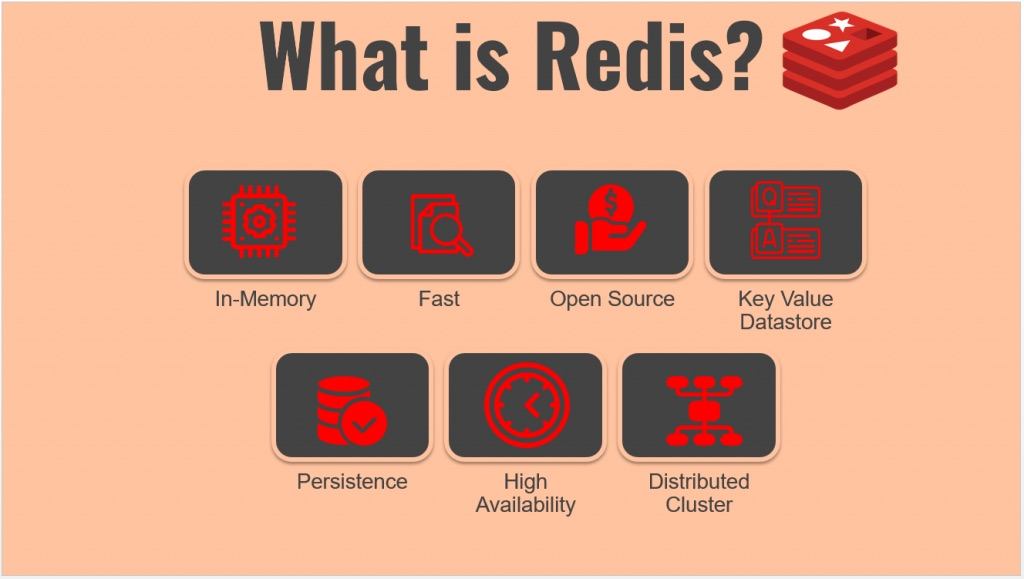
\includegraphics[width = 1\textwidth]{redis-features}
	\caption{Tính năng của Redis}
\end{figure}

\textbf{Performance}

Tất cả dữ liệu Redis nằm trong bộ nhớ, cho phép truy cập dữ liệu có độ trễ thấp và thông lượng cao. Không giống như cơ sở dữ liệu truyền thống, kho lưu trữ dữ liệu trong bộ nhớ không yêu cầu chuyển tới đĩa, giảm độ trễ của động cơ xuống micro giây. Do đó, các kho lưu trữ dữ liệu trong bộ nhớ có thể hỗ trợ nhiều thao tác hơn và thời gian phản hồi nhanh hơn. Kết quả là mang lại hiệu suất cực nhanh với các thao tác đọc và ghi trung bình chỉ mất chưa đến một phần nghìn giây và hỗ trợ hàng triệu thao tác mỗi giây.

\textbf{Cấu trúc dữ liệu linh hoạt}

Không giống như các kho dữ liệu khóa-giá trị khác cung cấp cấu trúc dữ liệu hạn chế, Redis có rất nhiều cấu trúc dữ liệu để đáp ứng nhu cầu ứng dụng của bạn. Các kiểu dữ liệu của Redis bao gồm:

\begin{figure}[H]
	\centering
	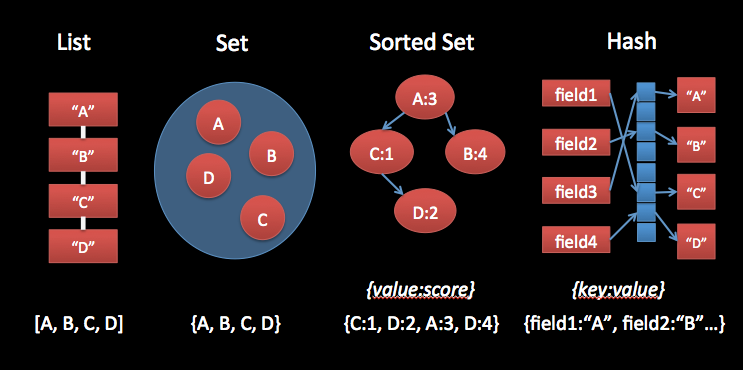
\includegraphics[width = 1\textwidth]{redis-data-structures}
	\caption{Cấu trúc dữ liệu của Redis}
\end{figure}

\begin{itemize}
	\bfitem{Strings}{dữ liệu văn bản hoặc dữ liệu nhị phân có kích thước lên đến 512MB}
	\bfitem{Lists}{tập hợp các Chuỗi theo thứ tự chúng được thêm vào}
	\bfitem{Sets}{một tập hợp các chuỗi không có thứ tự với khả năng giao nhau, kết hợp và khác các loại Bộ khác}
	\bfitem{Sorted Sets }{Các bộ được sắp xếp theo một giá trị}
	\bfitem{Hashes}{một cấu trúc dữ liệu để lưu trữ danh sách các trường và giá trị}
	\bfitem{Bitmap}{một kiểu dữ liệu cung cấp các hoạt động ở mức bit}
	\bfitem{HyperLogLogs}{cấu trúc dữ liệu xác suất để ước tính các mục duy nhất trong tập dữ liệu}
	\bfitem{Streams}{cấu trúc dữ liệu nhật ký Hàng đợi tin nhắn}
	\bfitem{Geospatial}{mục nhập dựa trên kinh độ / vĩ độ Bản đồ, "lân cận"}
	\bfitem{JSON}{một đối tượng lồng nhau, bán cấu trúc của các giá trị được đặt tên hỗ trợ số, chuỗi, Boolean, mảng và các đối tượng khác}
\end{itemize}

\textbf{Đơn giản và dễ sử dụng}

Redis cho phép bạn viết mã phức tạp truyền thống với ít dòng hơn, đơn giản hơn. Với Redis, bạn viết ít dòng mã hơn để lưu trữ, truy cập và sử dụng dữ liệu trong các ứng dụng của mình. Sự khác biệt là các nhà phát triển sử dụng Redis có thể sử dụng cấu trúc lệnh đơn giản trái ngược với các ngôn ngữ truy vấn của cơ sở dữ liệu truyền thống. Ví dụ: bạn có thể sử dụng cấu trúc dữ liệu băm Redis để di chuyển dữ liệu đến kho dữ liệu chỉ với một dòng mã. Một tác vụ tương tự trên kho dữ liệu không có cấu trúc dữ liệu băm sẽ yêu cầu nhiều dòng mã để chuyển đổi từ định dạng này sang định dạng khác. Redis đi kèm với cấu trúc dữ liệu gốc và nhiều tùy chọn để thao tác và tương tác với dữ liệu của bạn. Hơn một trăm ứng dụng khách mã nguồn mở có sẵn cho các nhà phát triển Redis. Các ngôn ngữ được hỗ trợ bao gồm Java, Python, PHP, C, C++, C\#, JavaScript, Node.js, Ruby, R, Go và nhiều ngôn ngữ khác.

\textbf{Nhân rộng và bền bỉ}

Redis sử dụng kiến trúc bản sao chính và hỗ trợ sao chép không đồng bộ, nơi dữ liệu có thể được sao chép sang nhiều máy chủ bản sao. Điều này cung cấp hiệu suất đọc được cải thiện (vì các yêu cầu có thể được phân chia giữa các máy chủ) và khôi phục nhanh hơn khi máy chủ chính gặp sự cố. Để bền bỉ, Redis hỗ trợ sao lưu theo thời gian (sao chép tập dữ liệu Redis vào đĩa).

Redis không được xây dựng để trở thành một cơ sở dữ liệu bền và nhất quán. Nếu bạn cần một cơ sở dữ liệu bền, tương thích với Redis, hãy xem xét Amazon MemoryDB cho Redis. Bởi vì MemoryDB sử dụng nhật ký giao dịch lâu dài để lưu trữ dữ liệu trên nhiều Vùng khả dụng (AZ), bạn có thể sử dụng nó làm cơ sở dữ liệu chính của mình. MemoryDB được xây dựng có mục đích cho phép các nhà phát triển sử dụng API Redis mà không phải lo lắng về việc quản lý bộ nhớ cache, cơ sở dữ liệu riêng biệt hoặc cơ sở hạ tầng bên dưới.

\textbf{Tính khả dụng và khả năng mở rộng cao}

Redis cung cấp một kiến trúc bản sao chính trong một nút chính hoặc một cấu trúc liên kết nhóm. Điều này cho phép bạn xây dựng các giải pháp có tính khả dụng cao, cung cấp hiệu suất và độ tin cậy nhất quán. Khi bạn cần điều chỉnh kích thước cụm của mình, các tùy chọn khác nhau để mở rộng và mở rộng quy mô trong hoặc ngoài cũng có sẵn. Điều này cho phép cụm của bạn phát triển theo nhu cầu của bạn.

\textbf{Mã nguồn mở}

Redis là một dự án mã nguồn mở được hỗ trợ bởi một cộng đồng sôi động, bao gồm AWS. Không có nhà cung cấp hoặc công nghệ nào bị khóa vì Redis dựa trên các tiêu chuẩn mở, hỗ trợ các định dạng dữ liệu mở và có một tập hợp khách hàng phong phú.

\subsubsection{Ứng dụng của Redis}

\begin{figure}[H]
	\centering
	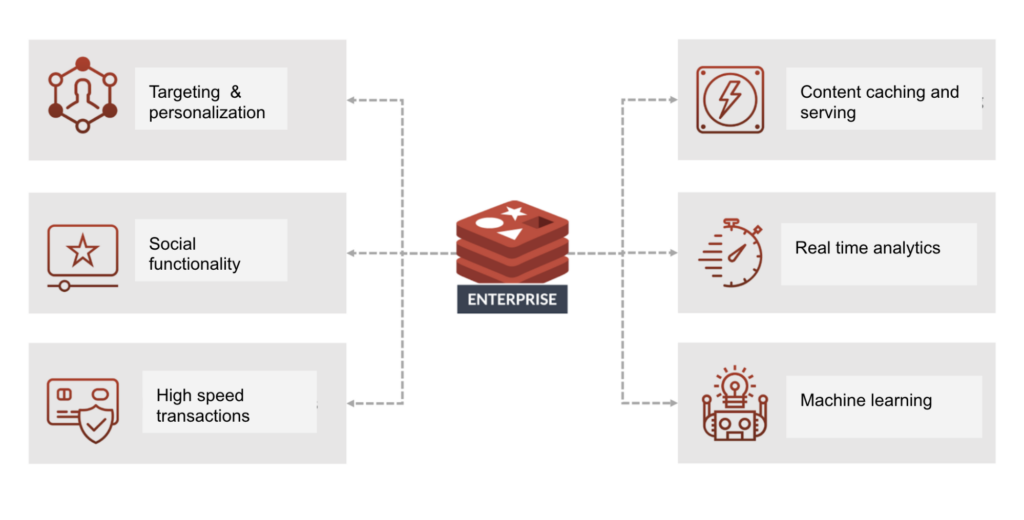
\includegraphics[width = 1\textwidth]{redis-use-cases}
	\caption{Ứng dụng của Redis}
\end{figure}

\textbf{Bộ nhớ đệm}

Redis là một lựa chọn tuyệt vời để triển khai bộ nhớ đệm trong bộ nhớ sẵn có cao để giảm độ trễ truy cập dữ liệu, tăng thông lượng và giảm tải cơ sở dữ liệu và ứng dụng NoSQL hoặc cơ sở dữ liệu quan hệ của bạn. Redis có thể phân phát các mặt hàng được yêu cầu thường xuyên ở thời gian phản hồi dưới mili giây và cho phép bạn dễ dàng mở rộng quy mô để có tải cao hơn mà không tăng phần phụ trợ tốn kém hơn. Bộ nhớ đệm kết quả truy vấn cơ sở dữ liệu, bộ nhớ đệm phiên liên tục, bộ nhớ đệm trang web và bộ nhớ đệm của các đối tượng được sử dụng thường xuyên như hình ảnh, tệp và siêu dữ liệu đều là những ví dụ phổ biến về bộ nhớ đệm với Redis.

\textbf{Trò chuyện, nhắn tin và hàng đợi}

Redis hỗ trợ Pub / Sub với tính năng so khớp mẫu và nhiều cấu trúc dữ liệu khác nhau như danh sách, tập hợp được sắp xếp và băm. Điều này cho phép Redis hỗ trợ các phòng trò chuyện hiệu suất cao, luồng bình luận trong thời gian thực, nguồn cấp dữ liệu mạng xã hội và giao tiếp liên máy chủ. Cấu trúc dữ liệu Redis List giúp dễ dàng triển khai một hàng đợi nhẹ. Danh sách cung cấp các hoạt động nguyên tử cũng như khả năng chặn, làm cho chúng phù hợp với nhiều ứng dụng khác nhau yêu cầu trình môi giới thông điệp đáng tin cậy hoặc danh sách vòng tròn.

\textbf{Bảng thành tích}

Redis là một lựa chọn phổ biến trong số các nhà phát triển trò chơi đang tìm cách xây dựng bảng xếp hạng thời gian thực. Chỉ cần sử dụng cấu trúc dữ liệu Redis Sorted Set, cung cấp tính duy nhất của các phần tử trong khi vẫn duy trì danh sách được sắp xếp theo điểm số của người dùng. Việc tạo danh sách được xếp hạng theo thời gian thực cũng dễ dàng như việc cập nhật điểm của người dùng mỗi khi nó thay đổi. Bạn cũng có thể sử dụng Bộ đã sắp xếp để xử lý dữ liệu chuỗi thời gian bằng cách sử dụng dấu thời gian làm điểm số.

\textbf{Lưu trữ session}

Redis như một kho lưu trữ dữ liệu trong bộ nhớ với tính khả dụng cao và bền bỉ là lựa chọn phổ biến của các nhà phát triển ứng dụng để lưu trữ và quản lý dữ liệu phiên cho các ứng dụng quy mô internet. Redis cung cấp độ trễ dưới mili giây, quy mô và khả năng phục hồi cần thiết để quản lý dữ liệu phiên, chẳng hạn như hồ sơ người dùng, thông tin đăng nhập, trạng thái phiên và cá nhân hóa người dùng cụ thể.

\textbf{Phát trực tuyến đa phương tiện}

Redis cung cấp một kho lưu trữ dữ liệu trong bộ nhớ, nhanh chóng để cung cấp năng lượng cho các trường hợp sử dụng phát trực tiếp. Redis có thể được sử dụng để lưu trữ siêu dữ liệu về hồ sơ của người dùng và lịch sử xem, thông tin xác thực / mã thông báo cho hàng triệu người dùng và tệp kê khai để cho phép CDN truyền video tới hàng triệu người dùng thiết bị di động và máy tính để bàn cùng một lúc.

\textbf{Không gian địa lý}

Redis cung cấp các cấu trúc và toán tử dữ liệu trong bộ nhớ được xây dựng có mục đích để quản lý dữ liệu không gian địa lý theo thời gian thực ở quy mô và tốc độ. Các lệnh như GEOADD, GEODIST, GEORADIUS và GEORADIUSBYMEMBER để lưu trữ, xử lý và phân tích dữ liệu không gian địa lý trong thời gian thực giúp không gian địa lý trở nên dễ dàng và nhanh chóng với Redis. Bạn có thể sử dụng Redis để thêm các tính năng dựa trên vị trí như thời gian lái xe, khoảng cách lái xe và các điểm ưa thích vào ứng dụng của bạn.

\textbf{Học máy}

Các ứng dụng hướng dữ liệu hiện đại yêu cầu máy học để xử lý nhanh chóng một khối lượng lớn, sự đa dạng và tốc độ của dữ liệu cũng như tự động hóa việc ra quyết định. Đối với các trường hợp sử dụng như phát hiện gian lận trong trò chơi và dịch vụ tài chính, đặt giá thầu thời gian thực trong công nghệ quảng cáo và mai mối trong việc hẹn hò và chia sẻ chuyến đi, khả năng xử lý dữ liệu trực tiếp và đưa ra quyết định trong vòng hàng chục mili giây là vô cùng quan trọng. Redis cung cấp cho bạn một kho lưu trữ dữ liệu trong bộ nhớ nhanh chóng để xây dựng, đào tạo và triển khai các mô hình học máy một cách nhanh chóng.

\textbf{Phân tích thời gian thực}

Redis có thể được sử dụng với các giải pháp phát trực tuyến như Apache Kafka và Amazon Kinesis như một kho lưu trữ dữ liệu trong bộ nhớ để nhập, xử lý và phân tích dữ liệu thời gian thực với độ trễ dưới mili giây. Redis là một lựa chọn lý tưởng cho các trường hợp sử dụng phân tích thời gian thực như phân tích phương tiện truyền thông xã hội, nhắm mục tiêu quảng cáo, cá nhân hóa và IoT.

% \subsection{Test Driven Development (TDD)}
